\chapter[Extraction des caractéristiques]{Extraction des caractéristiques visuelles}
\label{chap:sift}

\section{Introduction}
\newtheorem{mydef}{Définition}
\begin{mydef}
\textbf{Caractéristique visuelle} \\
Une caractéristique d'une image est définie comme une abstraction des informations visuelles de l'image qui sont sélectionnée pour des tâches de calcul reliées à une certaine application (par ex : classification d'images, recherche d'images).
\end{mydef}

Les caractéristiques sont extraites soit globalement sur une image entière, soit sur une petite groupe de pixel (une région) d'une image. Le résultat d'une étape d'extraction de caractéristiques (globales ou locales) est appelé \textit{descripteur de caractéristiques.}

\begin{mydef}
\textbf{Descripteur de caractéristiques} \\
Nous appelons la description mathématique d'une image ou une région locale de l'image après une étape d'extraction de caractéristiques sont \textbf{descripteur de caractéristiques}
\end{mydef}

Les descripteurs se présentent normalement sous forme d'une vecteur dans un espace vectoriel, $\mathbb{R}^D$, appelé \textit{l'espace de caractéristiques}. \\

Dans le cas d'une extraction globale, on récupère une seule descripteur par image tandis qu'une description locale permet d'obtenir d'un ensemble de descripteur locaux pour une image. \\

Jusqu'à maintenant, les cherches se basent plusieurs types de caractéristiques pour la classification ou la reconnaissance d'images. Nous pouvons lister quelques types de caractéristiques les plus couramment utilisées pour calculer des descripteur : \textit{la couleur, la texture, la forme, les points d'intérêt et les relations spatiales} qui sont décrit dans \cite{khang09}.\\

\section{Description locale des images}
Afin d'obtenir des descripteur locaux à partir une image, on commence par extraire des régions. La façon la plus simple est d'utiliser une \textit{partition} qui découpe l'image en rectangles ou en cercles de même taille. Une telle partition simple ne génère pas de région perceptuelle-ment significatives mais c'est une manière simple d'obtenir des caractéristiques globales de l'image avec une résolution plus fine. Dans la lecture, nous trouvons que les deux approches les plus utilisées pour localiser les région d'intérêt dans l'image : l'une fournit des régions qui se chevauchent (détection des points d'intérêt) et l'autre segmente l'image en région sans intersection (segmentation d'image)\cite{khang09}. La première approche est efficace pour la classification d'images, donc, dans cette section nous décrivons la première approche.\\[0.5cm]
\textbf{Détection des points d'intérêt}\\
Les points d'intérêt sont traditionnellement utilisés pour la \textit{stéréo vision} mais sont utilisés aussi dans la classification d'images. Ils sont déterminés de manière telle qu'un point trouvé dans une image sera aussi trouvé dans une autre image qui diffère légèrement de la première. La signification de tels points spéciaux est due à leur représentation compacte des régions importantes de l'image qui conduit à une indexation efficace, et à leur pouvoir discriminant surtout dans la recherche d'objets.\\

Un des premiers travaux sur ce sujet \cite{sm97} utilise un détecteur de Harris \cite{hs88} pour localiser des points d'intérêt invariants à la rotation. Dans \cite{dsh00}, les auteurs montrent que les descripteurs ne peuvent pas être invariants au changement d'échelle si les points d'intérêt extraits ne sont pas invariants eux même au changement d'échelle. Par conséquent, plusieurs détecteurs ont été proposé pour obtenir l'invariance au changement d'échelle des points d'intérêt \cite{lin98, low99, ms01, low04}. La sélection automatique de l'échelle est effectuer en choisissant les \textit{extrema} d'une fonction de l'échelle (par ex. laplacien normalisé, différence de gaussiennes).\\[0.5cm]
\textbf{Caractérisation des points d'intérêt}\\
Après avoir détecté des points d'intérêt, pour les utiliser, il faut caractériser la région autour de ces points. La caractérisation d'un point d'intérêt est calculée, à une échelle choisie, sur la région autour de ce point. Différents descripteurs ont été proposés dans la littérature : \textit{Shape context} \cite{bmp02}, \textit{Scale Invariant Feature Transform (SIFT)} \cite{low04}, \textit{PCA-SIFT} \cite{ks04}, \textit{Gradient Location and Orientation Histogram (GLOH)} \cite{ms05}. Parmi des descripteurs listés, le descripteur SIFT est le plus utilisé \cite{khang09}. Dans ce travail, nous concentrerons au descripteur SIFT, donc, nous décrivons ce descripteur et cette méthode dans la partie ci-dessous.

\section{Méthode SIFT (Scale-invariant feature transform)}
\subsection{Introduction}
Dans la lecture, nous trouvons qu'on traduit en français "transformation de caractéristiques visuelles invariante à l'échelle". SIFT est une méthode utilisé dans le domaine de la vision par ordinateur pour détecter et identifier les éléments similaires entre différentes images numériques (éléments de paysages, objets, personnes, etc.). Cette méthode a été développé en 1999 par le chercheur David Lowe \cite{low99}.\\

L'étape fondamentale de la méthode SIFT consiste à calculer les \textit{descripteurs SIFT} des images à étudier. Il s'agit d'informations numériques dérivées de l'analyse locale d'une image et qui caractérisent le contenu visuel de cette image de la façon la plus indépendante possible de l'échelle, du cadrage, de l'angle d'observation et de l'exposition (luminosité) \cite{low99}.\\

La méthode proposée par Lowe comprend deux parties \cite{low04}~:
\begin{enumerate}
\item un algorithme de détection de caractéristiques et de calcul de descripteurs
\item un algorithme de mise en correspondance proprement dit
\end{enumerate}
De ces deux aspects, le premier est celui qui a le plus assuré la popularité de la méthode \cite{mt10}. La deuxième permet d'utiliser le résultat de la première partie pour l'usage de la méthode. Dans notre travail, nous utilisons la méthode SIFT comme un résultat de base. C'est à dire, nous n'utilisons que la première partie de la méthode.\\

La première partie, partie de détection de caractéristiques et de calculer des descripteurs comprend 4 étapes principales \cite{low99, low04}~:
\begin{enumerate}
\item Détection d'extrema dans l'espace des échelles.
\item Localisation précise de points d'intérêt
\item Assignation d'orientation
\item Descripteur de point d'intérêt
\end{enumerate}
Nous décrivons tout de suite pas à pas ces étapes.

\subsection{Détection d'extrema dans l'espace des échelles}
La détection s'effectue dans un espace discret (espace des échelles ou \textit{scale space} en anglais) qui comporte trois dimensions : les coordonnées cartésiennes $x$ et $y$ et le facteur d'échelle $\sigma$. Le gradient de facteur d'échelle $\sigma$ (noté $L$) est le résultat de la convolution d'une image $I$ par un filtre gaussien $G$ de paramètre d'échelle $\sigma$, soit \cite{low04} :

\begin{equation}
L \left( x, y, \sigma \right) = G \left( x, y, \sigma \right) * I \left( x, y \right)
\end{equation}
Et
\[
G \left( x, y, \sigma \right) = \frac{1}{2\pi\sigma^2}
\]

Cette convolution a pour effet de lisser l'image originale $I$ de telle sorte que les détails trop petits, c'est-à-dire de rayon inférieur à \footnote{ Ici comme dans la littérature scientifique en général, le facteur d'échelle – paramètre du filtre gaussien $\sigma$ – est assimilé à une distance en pixels sur l'image, que l'on pourrait appeler rayon associé $r$. En fait, ils sont proportionnels ($r = \alpha \sigma$), avec un facteur $\alpha$ qui varie généralement entre 3 et 4 selon les auteurs. Il est tout simplement lié au nombre de coefficients au-delà duquel les valeurs de la gaussienne deviennent négligeables.}, sont estompés. Par conséquent, la détection des objets de dimension approximativement égale à $\sigma$ se fait en étudiant l'image appelée différences de gaussiennes (en anglais difference of gaussians, DoG) définie comme suit :
\begin{equation}
D \left( x, y, \sigma \right) = L \left( x, y, k\sigma \right) - L \left( x, y, \sigma \right)
\end{equation}
Ou
\[
D \left( x, y, \sigma \right) = (G \left( x, y, k\sigma \right) - G \left( x, y, \sigma \right)) * I \left( x, y \right)
\]

où $k$ est un paramètre fixe de l'algorithme qui dépend de la finesse de la discrétisation de l'espace des échelles voulue \cite{low04}.\\

Pour chaque octave de l'espace des échelle, l'image initiale répétée est fait la convolution avec gaussiennes pour produire l'ensemble des images de l'espace des échelle (image ci-dessous, à gauche). Images gaussiennes adjacentes sont soustraites
pour produire les images de différence de gaussienne sur la droite. Après chaque octave, l'image Gaussian est sous-échantillonnée par un facteur de 2, et le processus est répété pour toutes les échelle.

\begin{figure}[ht!]
\centering
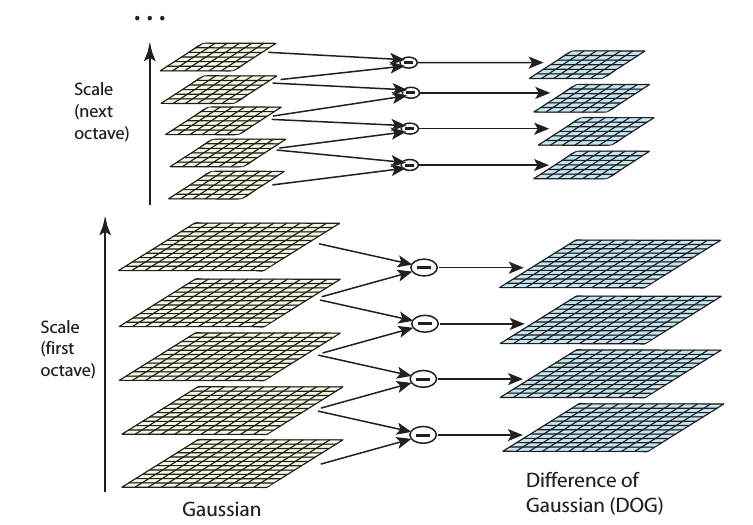
\includegraphics[width=150mm]{images/dog}
\caption{Différence de Gausienne \cite{low04}}
\label{overflow}
\end{figure}

Un point d'intérêt candidat ($x,y,\sigma$) est défini comme un point où un extremum du DoG est atteint par rapport à ses voisins immédiats, c'est-à-dire sur l'ensemble contenant 26 autres points défini par~:
\[
\{ D \left( x + \delta_x, y + \delta_y, s \sigma \right), \delta_x \in \{-1, 0, 1\}, \delta_y \in \{-1,0, 1\}, s \in \{k^{-1}, 1, k\} \} 
\]
On peut voir l'image ci-dessous pour être facile à comprendre
\begin{figure}[ht!]
\centering
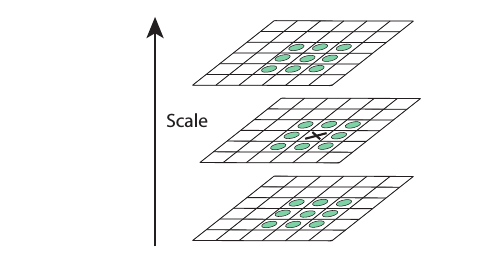
\includegraphics[width=100mm]{images/select_point}
\caption{\cite{low04} Le maxima et le minima des images de différence de gaussienne sont détectés en comparant une
pixel (marqué X) à ses 26 voisins dans les régions de 3x3 aux échelles actuels et adjacents (marqué avec des cercles).}
\label{overflow}
\end{figure}

\pagebreak
\subsection{Localisation précise de points d'intérêt}
L'étape de détection d'extremums produit en général un grand nombre de points-clés candidats, dont certains sont instables. De plus, leur localisation, en particulier aux échelles les plus grandes (autrement dit dans les octaves supérieures de la pyramide où la résolution est plus faible) reste approximative. De ce fait, des traitements supplémentaires sont appliqués, pour un objectif double : d'une part, reconverger la position des points pour améliorer la précision sur $x$, $y$ et $\sigma$, d'autre part, éliminer les points de faible contraste ou situés sur des arêtes de contour à faible courbure et donc susceptibles de "glisser" facilement.

\subsection{Assignation d'orientation}
L'étape d'assignation d'orientation consiste à attribuer à chaque point-clé une ou plusieurs orientations déterminées localement sur l'image à partir de la direction des gradients dans un voisinage autour du point. Dans la mesure où les descripteurs sont calculés relativement à ces orientations, cette étape est essentielle pour garantir l'invariance de ceux-ci à la rotation : les mêmes descripteurs doivent pouvoir être obtenus à partir d'une même image, quelle qu'en soit l'orientation\cite{low04}.

Pour un point-clé donné ( $x_0$, $y_0$, $\sigma_0$ ), le calcul s'effectue sur $L ( x, y, \sigma_0 )$, à savoir le gradient de la pyramide dont le paramètre est le plus proche du facteur d'échelle du point. De cette façon, le calcul est également invariant à l'échelle. À chaque position dans un voisinage du point-clé, on estime le gradient par différences finies symétriques, puis son amplitude (c.-à-d. sa norme) $m ( x, y )$, et son orientation $\theta ( x, y )$ \cite{low04}~:

\begin{equation}
m \left( x, y \right) = \sqrt{\bigl( L \left( x+1, y \right) - L \left( x-1, y \right) \bigr)^2 + \bigl( L \left( x, y+1 \right) - L \left( x, y-1 \right) \bigr)^2}
\end{equation}

\begin{equation}
\theta \left( x, y \right) = \tan^{-1}\left(\frac{L \left( x, y+1 \right) - L \left( x, y-1 \right)}{L \left( x+1, y \right) - L \left( x-1, y \right)} \right)
\forall\left(x, y\right) \hbox{ dans un voisinage de } \left(x_0, y_0\right)
\end{equation}

Un histogramme des orientations sur le voisinage est réalisé avec 36 intervalles, couvrant chacun 10 degrés d'angle. L'histogramme est doublement pondéré : d'une part, par une fenêtre circulaire gaussienne de paramètre égal à 1,5 fois le facteur d'échelle du point-clé $\sigma_0$, d'autre part, par l'amplitude de chaque point. Les pics dans cet histogramme correspondent aux orientations dominantes. Toutes les orientations dominantes permettant d'atteindre au moins 80\% de la valeur maximale sont prises en considération, ce qui provoque si nécessaire la création de points-clés supplémentaires ne différant que par leur orientation principale\cite{low04}.

\begin{figure}[ht!]
\centering
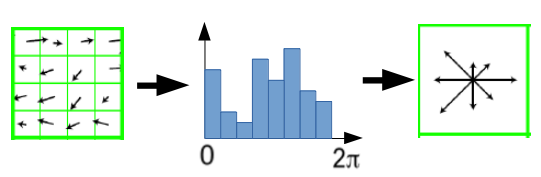
\includegraphics[width=100mm]{images/sift_hist}
\caption{Illustration de la construction de l'histogramme des orientations}
\label{overflow}
\end{figure}

À l'issue de cette étape, un point-clé est donc défini par quatre paramètres $( x, y, \sigma, \theta )$. Il est à noter qu'il est parfaitement possible qu'il y ait sur une même image plusieurs points-clés qui ne différent que par un seul de ces quatre paramètres (le facteur d'échelle ou l'orientation, par exemple).


\subsection{Descripteur de point d'intérêt}
Une fois les points-clés, associés à des facteurs d'échelles et à des orientations, détectés et leur invariance aux changements d'échelles et aux rotations assurée, arrive l'étape de calcul des vecteurs descripteurs, traduisant numériquement chacun de ces points-clés. À cette occasion, des traitements supplémentaires vont permettre d'assurer un surcroît de pouvoir discriminant en rendant les descripteurs invariants à d'autres transformations telles que la luminosité, le changement de point de vue 3D, etc. Cette étape est réalisée sur l'image lissée avec le paramètre de facteur d'échelle le plus proche de celui du point-clé considéré\cite{low04}.
\begin{figure}[ht!]
\centering
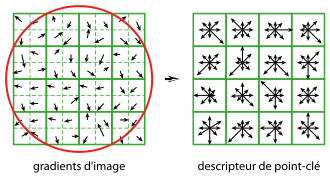
\includegraphics[width=100mm]{images/siftdescriptor}
\caption{Construction d'un descripteur SIFT}
\label{overflow}
\end{figure}

Autour de ce point, on commence par modifier le système de coordonnées local pour garantir l'invariance à la rotation, en utilisant une rotation d'angle égal à l'orientation du point-clé, mais de sens opposé. On considère ensuite, toujours autour du point-clé, une région de $16x16$ pixels, subdivisée en $4x4$ zones de $4x4$ pixels chacune. Sur chaque zone est calculé un histogramme des orientations comportant 8 intervalles. En chaque point de la zone, l'orientation et l'amplitude du gradient sont calculés comme précédemment. L'orientation détermine l'intervalle à incrémenter dans l'histogramme, ce qui se fait avec une double pondération par l'amplitude et par une fenêtre gaussienne centrée sur le point clé, de paramètre égal à 1,5 fois le facteur d'échelle du point-clé\cite{low04}.\\

Ensuite, les 16 histogrammes à 8 intervalles chacun sont concaténés et normalisés. Dans le but de diminuer la sensibilité du descripteur aux changements de luminosité, les valeurs sont plafonnées à 0,2 et l'histogramme est de nouveau normalisé, pour finalement fournir le descripteur SIFT du point-clé, de dimension 128.

\section{Méthode BoW (Bag of word)}
La représentation par sac de mots \textit{(ou bag of words en anglais)} est une description de document (texte, image, ...) très utilisée en recherche d'information. Spécialement, dans la classification d'images, cette méthode est largement utilisée après l'étape d'extraction des descripteurs. Dans DoW, les méthodes de cluster sont utilisées pour grouper des  descripteurs. Actuellement, la méthode K-moyenne (Kmeans)\cite{jm67} est beaucoup utilisée pour grouper des des descripteurs SIFT aux clusters, chaque cluster est considère comme un mot visuel, l'ensemble de mots visuels jouent le rôle d'un dictionnaire de mots visuels. Ensuite, BoW met chaque descripteur de chaque image au cluster qui est le plus proche( se base sur la distance entre chaque descripteur et sa future cluster ). Suite, chaque image est décrite comme un histogramme des mots. Cette méthode est décrite comme l'image ci-dessous.

\begin{figure}[ht!]
\centering
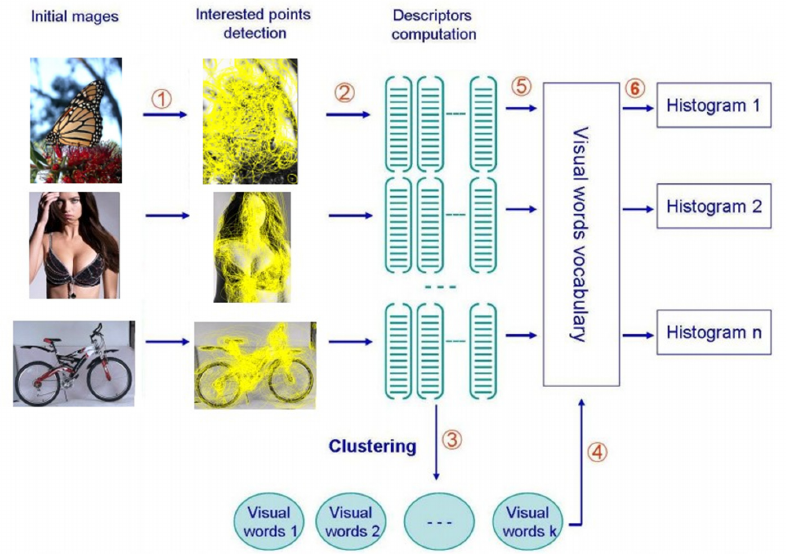
\includegraphics[width=160mm]{images/bow}
\caption{Model de BOW}
\label{overflow}
\end{figure}

\chapter{Apprentissage automatique}
\label{chap:sgd}

\section{Introduction}
L'apprentissage automatique (machine learning) est un domaine de l'intelligence artificielle, qui permet aux machines d'apprendre à partir des données. L'apprentissage automatique est la discipline scientifique concernée par le développement, l'analyse et l'implémentation de méthodes automatisables qui permettent à une machine d'évoluer autonome-ment grâce à un processus d'apprentissage, et ainsi de remplir des tâches qu'il est difficile ou impossible de remplir par des moyens algorithmiques plus classiques. Le problème ici est que la donnée d'observation est petite, elle ne peut pas comprendre tout l'ensemble de données d'entrées (tous les cas) qui est trop grande. Un programme d'apprentissage automatique doit généraliser des données limite afin de données des réactions intelligentes sur des nouveaux exemples.\\

\section{Méthode SVM (Support Vector Machine)}
Les machines à vecteurs de support (Support Vector Machine, SVM) sont un ensemble de techniques d'apprentissage supervisé destinées à résoudre des problèmes de classification et de régression. Dans cette section, nous ne parlons que SVM pour la classification concernant notre projet dans la pratique.\\

Supposons que l'on a le problème de classification. Le cas simple est le cas d'une fonction de classification linéaire comme dans l'image \ref{slines}. On a $m$ exemples d'entrées $x_1, x_2, ..., x_m$ dans l'espace de $N$ dimensions. Chaque exemple $x_i$ a un label $y_i$ : $y_1, y_2, ..., y_m$ $(y_i \in \{-1,1\})$. Plusieurs hyperplans peuvent séparer ces 2 classes, quel est l'hyperplan optimal ?

\begin{figure}[ht!]
\centering
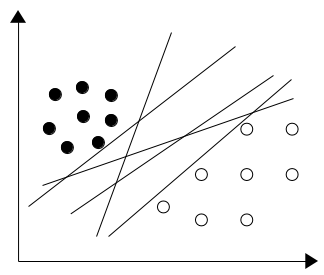
\includegraphics[width=55mm]{images/separating_lines}
\caption{Classification linéaire}
\label{slines}
\end{figure}

SVM cherche l'hyperplan optimal qui est défini comme l'hyperplan qui maximise la marge entre les échantillons et l'hyperplan séparateur. La marge est la distance entre l'hyperplan et les échantillons les plus proches. Ces derniers sont appelés \textit{vecteurs supports}. Dans l'espace de \textit{N} dimensions, l'hyperplan est défini par le vecteur $w=[w_1,w_2,...,w_n]$ et $b$. SVM cherche l'hyperplan $(w, b)$ pour classifier les données comme l'image \ref{max_margin} :

\begin{figure}[ht!]
\centering
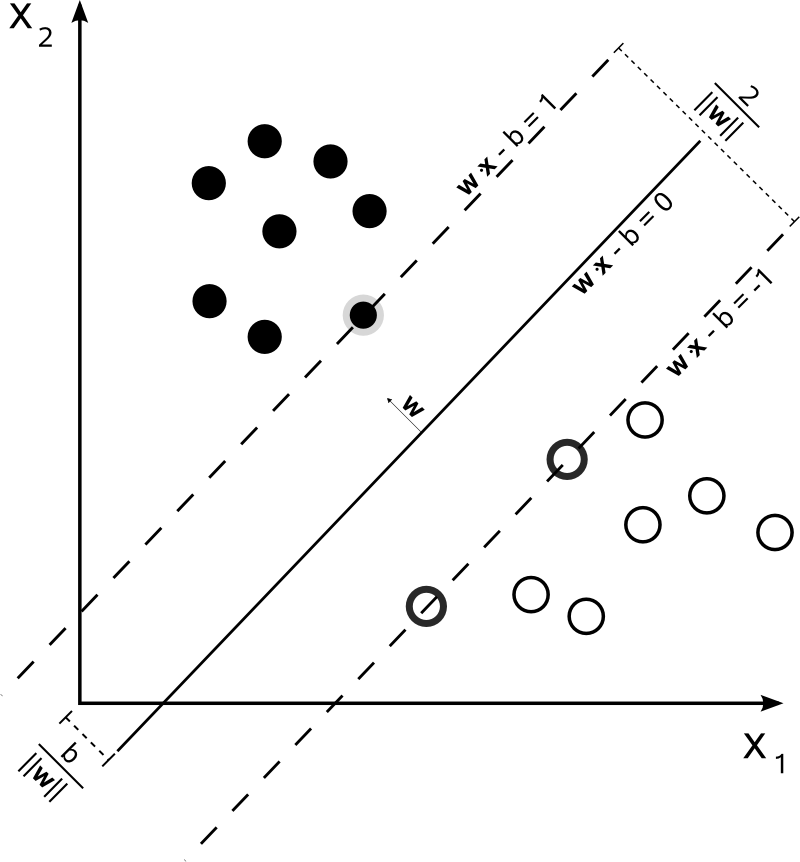
\includegraphics[width=55mm]{images/margin}
\caption{L'hyperplan optimal}
\label{max_margin}
\end{figure}

Après avoir trouvé $w$ et $b$, l'hyperplan optimal est défini : $x^T.w - b = 0$ et 2 supports hyperplans $x^T.w - b = 1$ et $x^T.w - b = -1$. Par rapport à 2 supports hyperplans parallèles (voir l'image \ref{max_margin}), la classification est réalisée grâce aux \ref{f1} et \ref{f2}.
\begin{equation}
x_i.w - b \geq +1, \Rightarrow y_i = 1
\label{f1}
\end{equation}

\begin{equation}
x_i.w - b \leq -1, \Rightarrow y_i = -1
\label{f2}
\end{equation}

La classification peut être expliqué : l'hyperplan supporte la classe \textit{\textbf{(+1)}} est l'hyperplan que les points qui a le label \textit{\textbf{(+1)}} au dessus de l'hyperplan. Comme ça, l'hyperplan supporte la classe \textit{\textbf{(-1)}} est l'hyperplan que les points qui a le label \textit{\textbf{(-1)}} au dessous de l'hyperplan. Par rapport aux \ref{f1} et \ref{f2}, on a le formule \ref{f3}

\begin{equation}
y_i.(x_i.w - b) \geq 1
\label{f3}
\end{equation}

Dans le cas où l'algorithme ne peut pas trouver $(w, b)$ satisfait le problème (les données sont inséparable), nous devons accepter des erreurs $z_i$. Chaque exemple $i$ est dans son vrais hyperplan, son erreur $z_i = 0$, sinon, son erreur $z_i$ est défini par la distance entre cet exemple et son hyperplan. Le formule \ref{f3} devient \ref{f4} :

\begin{equation}
y_i.(x_i.w - b) + z_i \geq 1
\label{f4}
\end{equation}

Nous trouvons que la classification est facile si l'on a trouvé $w$ et $b$. La difficulté de la méthode SVM est que comment trouver $w$ et $b$. Ce tache est réalisé après avoir trouvé la solution du programme de quadratique \ref{f5}.

\begin{equation}
\begin{split}
\mbox{min}\quad \Psi(w, b, z) = \frac{1}{2} ||w||^2 + c.\sum\limits_{i=1}^m z_i\quad \\ \mbox{s.t} \quad y_i.(x_i.w - b) + z_i \geq 1 \\ \mbox{and} \quad z_i \geq 0
\end{split}
\label{f5}
\end{equation}

Le problème d'optimisation quadratique \ref{f5} est un des problèmes d'optimisation qui est normalement recherché dans le domaine de mathématique d'optimisation. Pour l'implémentation ce problème, \cite{jp98} et \cite{cl01} ont la complexité de $O(N^2)$ (N est le nombre d'exemples). Ce sont des programmes les plus utilisés actuel.

\section{Méthode SVM avec SGD (Stochastic gradient descent)}
SVM standard est efficace mais la complicité est grande $(O(N^2))$, donc, c'est intraitable pour les larges données. La méthode SVM avec SGD (Stochastic Gradient Descent), ou pour plus simple, on appelle la méthode SGD est créées pour résoudre ce problème. SGD ne cherche pas la solution pour résoudre le problème du programme de quadratique \ref{f5}. Cette méthode ignore $b$  dans le formule \ref{f5}. Le contraint $y_i.(x_i.w - b) + z_i \geq 1$ peut être remplacé par : 

\begin{equation}
z_i \geq 1 - y_i.(x_i.w)
\label{f6}
\end{equation}

A partir du contraint \ref{f6} et $z_i \geq 0$, on peut écrire la function de perte :

\begin{equation}
z_i = max\lbrace0, 1 - y_i.(x_i.w)\rbrace
\label{f7}
\end{equation}

Donc, le programme de quadratique \ref{f5} peut remplacer par le formule \ref{f7} :

\begin{equation}
\mbox{min}\quad \Psi(w, x, y) = \frac{1}{2} ||w||^2 + \frac{1}{m}\sum\limits_{i=1}^m max\lbrace0, 1 - y_i.(x_i.w)\rbrace\quad
\label{f7}
\end{equation}

Cette méthode est proposée dans \cite{sss07}. Dans cette méthode, $w$ est mise à jour en T étapes avec une vitesse d'apprentissage $\eta$. A chaque étape $t$, SGD utilise un exemple $(x_i, y_i)$ aléatoire pour calculer le sous-gradient et met à jour $w_{t+1}$. 

\begin{equation}
w_{t+1} = w_t - \nabla_w{\Psi(w_t, x_i, y_i)}
\label{f8}
\end{equation}
\\

Cette algorithme est linéaire avec le nombre d'exemple. C'est la raison pour laquelle il est beaucoup plus vite que SVM standard. 

%Nous avons tester avec les données \textit{gisette} \cite{svmdata1} de 10 classes, 60.000 exemples et de 780 caractéristiques par exemple. 

\section{Méthode MC-SGD (Multi Class - Stochastic gradient descent)}
Plupart d'algorithme de SVM ne traite que le problème de 2 classes (binaire). Il existe plusieurs extensions d'une classification binaire afin de traiter le problème de multi-class classification. Actuellement, on a deux façons pour traiter ce problème. L'une considère directement à résoudre le problème de multi-classes \cite{ww99, yg07}. L'autre divise d'abord le problème en plusieurs problèmes de 2 classes et chaque problème de 2 classes est traité par la classification binaire comme one-versus-one \cite{vv95} et one-versus-all \cite{uk99}. En pratique, one-vs-one et one-vs-all sont beaucoup utilisés par leur simple.\\

\subsection{One-versus-one}
One-vs-one construit \textit{k(k-1)/2} (k est le nombre de classes) classificateurs, c'est à dire, il utilise tous les paires de classes différents pour l'apprentissage. La prédiction est réalisée par voter et la majorité classificateur va être choisi et la classe correspondant est la classe de prédiction. 


\begin{figure}[htbp!]
        \centering
        \begin{subfigure}[b]{0.5\textwidth}
                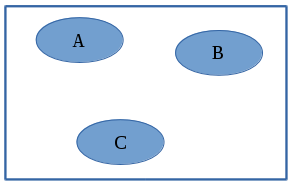
\includegraphics[width=\textwidth]{images/multiclass}
                \caption{Problème}
                \label{mclass}
        \end{subfigure}%
        ~ %add desired spacing between images, e. g. ~, \quad, \qquad, \hfill etc.
          %(or a blank line to force the subfigure onto a new line)
        \begin{subfigure}[b]{0.5\textwidth}
                \includegraphics[width=\textwidth]{images/1vs1c}
                \caption{one-vs-all}
                \label{1vs1c}
        \end{subfigure}
        \caption{Problème de multi-classes one-versus-one}\label{mulclass}
\end{figure}


L'image \ref{1vs1c} est comme un résumé de one-vs-one. Pour plus claire, nous vous listons les trois classificateurs de ces trois classes comme l'image \ref{1vs1detail}

\begin{figure}[htbp!]
        \centering
        \begin{subfigure}[b]{0.3\textwidth}
                \includegraphics[width=\textwidth]{images/classac}
                \caption{classe A vs classe C}
                \label{classac}
        \end{subfigure}%
        ~ %add desired spacing between images, e. g. ~, \quad, \qquad, \hfill etc.
          %(or a blank line to force the subfigure onto a new line)
        \begin{subfigure}[b]{0.3\textwidth}
                \includegraphics[width=\textwidth]{images/classab}
                \caption{classe A vs classe B}
                \label{classab}
        \end{subfigure}
        ~ %add desired spacing between images, e. g. ~, \quad, \qquad, \hfill etc.
          %(or a blank line to force the subfigure onto a new line)
        \begin{subfigure}[b]{0.30\textwidth}
                \includegraphics[width=\textwidth]{images/classbc}
                \caption{classe B vs classe C}
                \label{classbc}
        \end{subfigure}
        \caption{Problème de multi-classes one-versus-one détaillé}\label{1vs1detail}
\end{figure}


\subsection{One-versus-all}
One-vs-all construit \textit{k} classificateurs, à chaque classificateur \textit{c}, il divise la classes \textit{c} contre tous les restes. La classe de prédiction est la classe ayant la distance la plus courte entre son classificateur et l'exemple d'entrée.

\begin{figure}[H]
        \centering
        \begin{subfigure}[b]{0.5\textwidth}
                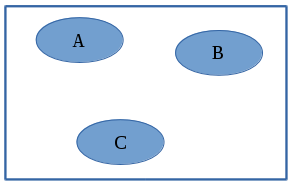
\includegraphics[width=\textwidth]{images/multiclass}
                \caption{Problème}
                \label{mclass}
        \end{subfigure}%
        ~ %add desired spacing between images, e. g. ~, \quad, \qquad, \hfill etc.
          %(or a blank line to force the subfigure onto a new line)
        \begin{subfigure}[b]{0.5\textwidth}
                \includegraphics[width=\textwidth]{images/1vsall}
                \caption{one-vs-all}
                \label{1vsall}
        \end{subfigure}
        \caption{Problème de multi-classes one-versus-all}\label{mulclass}
\end{figure}


L'image \ref{1vsall} est comme un résumé de one-vs-all. Pour plus claire, nous vous listons les trois classificateurs de ces trois classes comme l'image \ref{1vsalldetail}

\begin{figure}[H]
        \centering
        \begin{subfigure}[b]{0.3\textwidth}
                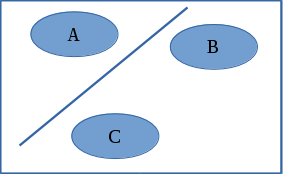
\includegraphics[width=\textwidth]{images/classa}
                \caption{classe A}
                \label{classa}
        \end{subfigure}%
        ~ %add desired spacing between images, e. g. ~, \quad, \qquad, \hfill etc.
          %(or a blank line to force the subfigure onto a new line)
        \begin{subfigure}[b]{0.3\textwidth}
                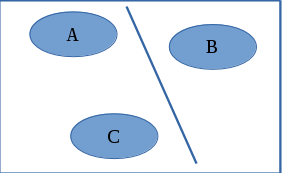
\includegraphics[width=\textwidth]{images/classb}
                \caption{class B}
                \label{classb}
        \end{subfigure}
        ~ %add desired spacing between images, e. g. ~, \quad, \qquad, \hfill etc.
          %(or a blank line to force the subfigure onto a new line)
        \begin{subfigure}[b]{0.30\textwidth}
                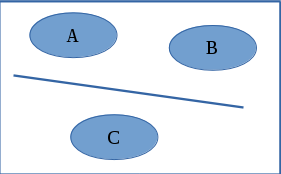
\includegraphics[width=\textwidth]{images/classc}
                \caption{class C}
                \label{classc}
        \end{subfigure}
        \caption{Problème de multi-classes one-versus-all détaillé}\label{1vsalldetail}
\end{figure}


Chaque méthode a l'avantage et l'inconvénient. One-vs-one est balancé mais il construit beaucoup de classificateurs. Par contre, one-vs-all construit moins classificateur mais il n'est pas balancé.